
\begin{frame}
  \titlepage
\end{frame}

\begin{frame}{Outline}

  \tableofcontents
  % You might wish to add the option [pausesections]

\end{frame}

% \begin{frame}{Outline}
% \begin{columns}
% \column{.5\textwidth}
%   \tableofcontents
%   % You might wish to add the option [pausesections]
% \column{.5\textwidth}
%   \begin{center}
% \begin{figure}[htbp]  
%   \begin{center}
%     \movie[width=40mm]{placeholder box}{6dofid_vid.avi}
%     %\includegraphics[]{}
%   \end{center}
%   %\caption{McFarland and Nereus (WHOI) during field deployment in 2011.}
% \end{figure}
% \end{center}

% \end{columns}

% \end{frame}

% \begin{frame}{temporalTest}
% \begin{itemize}
%   \item<1-> stuff
%   \item<2-> about
%   \item<3-> rigid body
% \end{itemize}
% \temporal<2>
% {

% one

% }{

% two

% }{

% three}
% \end{frame}

% Structuring a talk is a difficult task and the following structure
% may not be suitable. Here are some rules that apply for this
% solution: 

% - Exactly two or three sections (other than the summary).
% - At *most* three subsections per section.
% - Talk about 30s to 2min per frame. So there should be between about
%   15 and 30 frames, all told.

% - A conference audience is likely to know very little of what you
%   are going to talk about. So *simplify*!
% - In a 20min talk, getting the main ideas across is hard
%   enough. Leave out details, even if it means being less precise than
%   you think necessary.
% - If you omit details that are vital to the proof/implementation,
%   just say so once. Everybody will be happy with that.

\section{Introduction}
\subsection{Motivation}
\begin{frame}[t]{Motivation}
  Recent advances in Underwater Vehicle (UV) systems have enabled
  scientists and engineers to consider complex, multifaceted UV
  missions previously thought impractical or infeasible.

\uncover<6->{  \alert{Thesis Goal}: Develop improved
  {\bf state estimation}, {\bf parameter identification}, and
  {\bf control} algorithms.}
%    
    \begin{columns}
      \column{.45\textwidth}
\alt<1>{}{    \begin{center}
      \begin{figure}[htbp]
        \begin{center}
          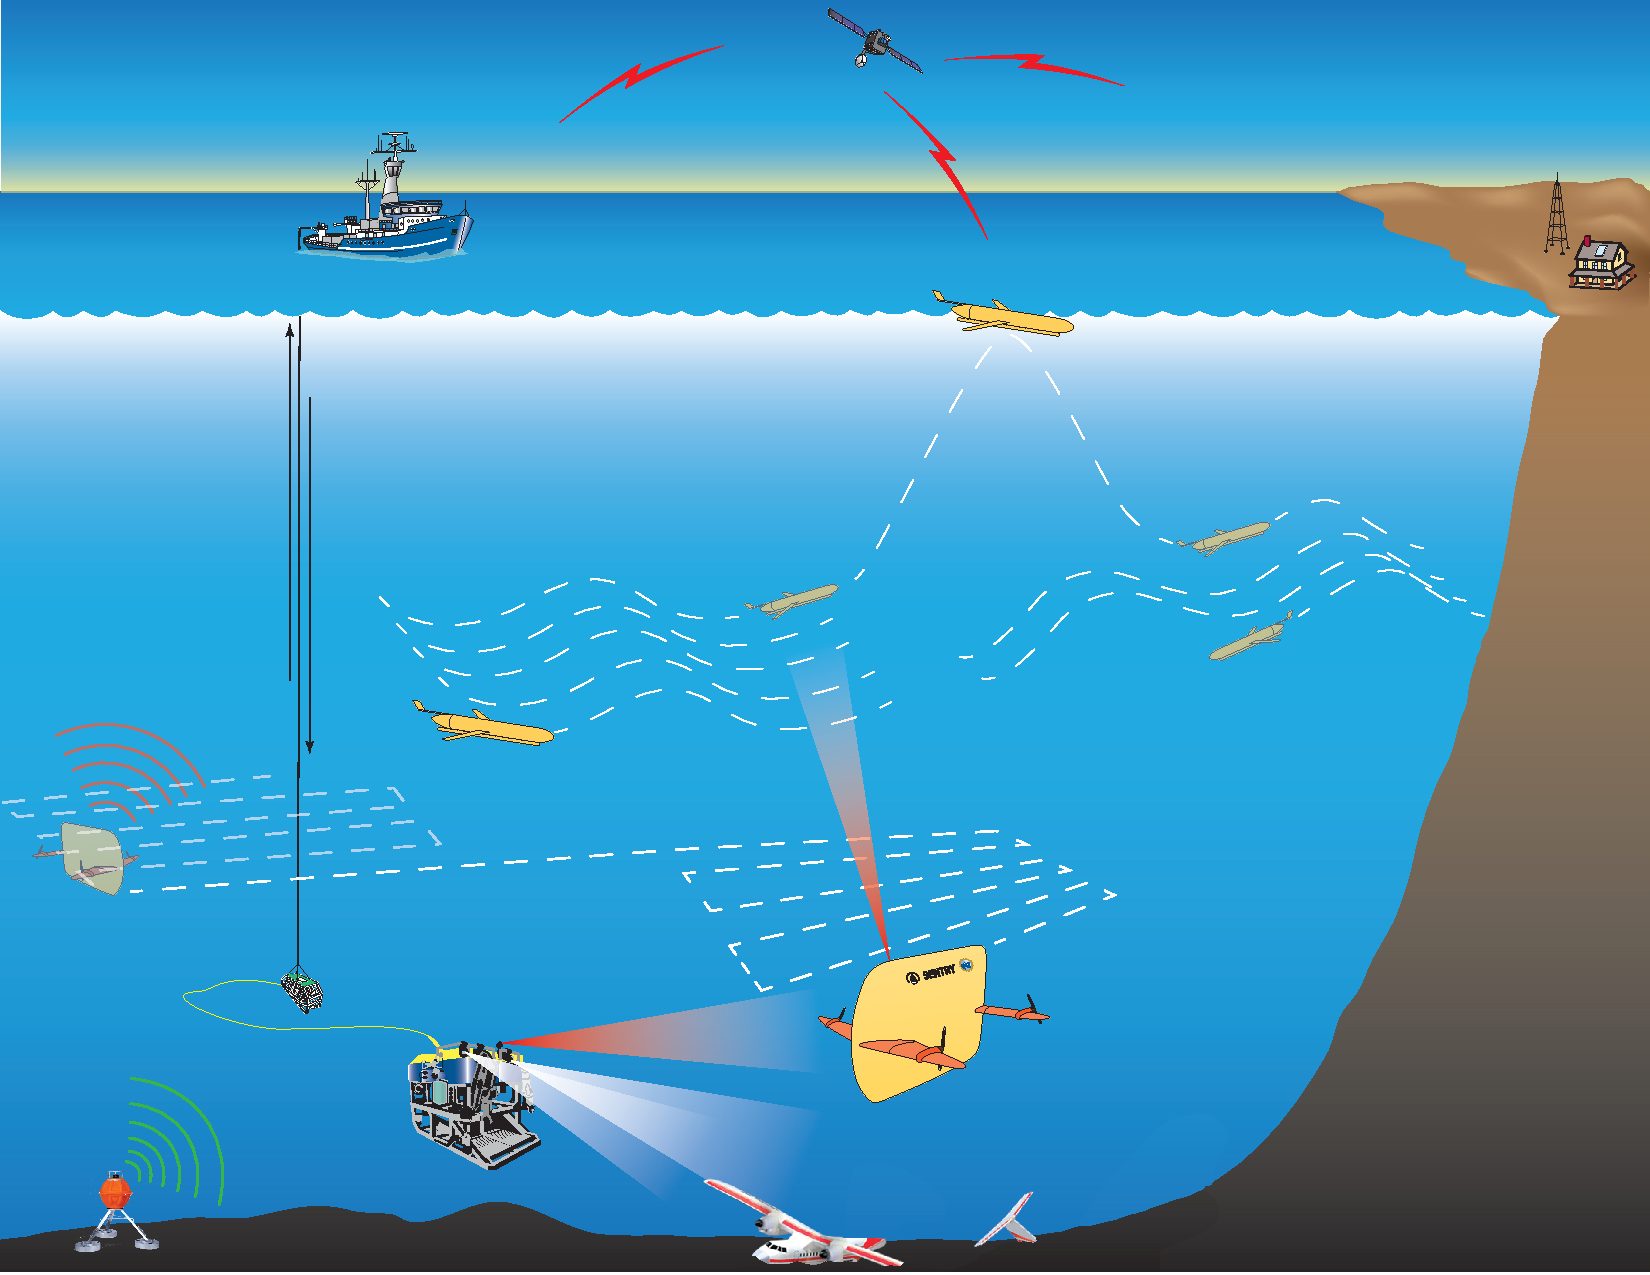
\includegraphics[width=1.1\textwidth]{./pres/images/Adaptive4}
%\caption{ Image credit: Paul Oberlander, WHOI. }
        \end{center}
      \end{figure}
    \end{center}
{\small Image credit: Paul Oberlander, WHOI.}}

  \column{.55\textwidth}

\alt<1-5>{
  \begin{itemize}
  \item<3-> UV teams for environmental monitoring
  \item<4-> Ship-based or on-shore operator monitoring and re-tasking of
    UVs
  \item<5-> Deployment of UVs in delicate or dynamic environments
  \end{itemize}
}{
  \begin{itemize}
  \item<7-> {\bf Improved State Estimation} algorithms can
    increase navigation accuracy while lowering UV cost.
  \item<8-> {\bf Improved Parameter Identification} algorithms enable
    remote operators to use forward simulation for mission planning
    and diagnose UV failure.
  \item<9-> {\bf Improved Control} algorithms enable increased precision
    of delicate or dynamic 6-degree-of-freedom
    (DOF) operation.
  \end{itemize}
}

 \end{columns}

\end{frame}

\subsection{Thesis Contributions}
\begin{frame}{Thesis Contributions}

{\small
{\setbeamercolor*{item}{fg=blue}
   \begin{columns}
      \column{.32\textwidth}
{\color{blue} \bf State Estimation:}
    \begin{center}
      \begin{figure}[t!]
        \begin{center}
          \includegraphics[width=\textwidth]{./pres/images/justGliders}
        \end{center}
      \end{figure}
    \end{center}
  \column{.75\textwidth}
%{\fontsize{7}{11}\selectfont
   \begin{itemize}
\item<1> 3-DOF Rotational Plant Velocity Observer %with stability analysis
\item<1> Simulation Study: 3-DOF Rotational Plant Velocity Observers
   \end{itemize}%}
\end{columns}}

{\color{OliveGreen}\rule{\linewidth}{4pt}
\setbeamercolor*{item}{fg=OliveGreen}
\vspace*{-5mm}
   \begin{columns}
      \column{.32\textwidth}
{\bf Parameter Identification:}
 %   \begin{center}
      \begin{figure}[t!]
        \begin{center}
          \includegraphics[width=\textwidth]{./pres/images/justSentry}
        \end{center}
      \end{figure}
%    \end{center}
  \column{.75\textwidth}
%{\tiny
\begin{itemize}
\item 3-DOF Rotational Dynamics Adaptive Identification (AID)
\item<1> Simulation Study: 3-DOF Rotational Plant AID
\item<1> {\it n}-link Open Kinematic Chain AID 
\item<1> 3-DOF UV Rotational Dynamics AID
\item<1> Experimental Evaluation: 3-DOF UV Rotational Dyn. AID
\item 6-DOF UV AID
\item Experimental Evaluation: 6-DOF UV AID
   \end{itemize}%}
\end{columns}}

{\color{red}\rule{\linewidth}{4pt}
\setbeamercolor*{item}{fg=red}
\vspace*{-2mm}
   \begin{columns}
      \column{.32\textwidth}
{\bf Trajectory-Tracking:}
    \begin{center}
      \begin{figure}[htbp]
        \begin{center}
          \includegraphics[width=\textwidth]{./pres/images/justJason}
        \end{center}
      \end{figure}
    \end{center}
  \column{.75\textwidth}
%{\tiny
\vspace*{-2mm}
   \begin{itemize}
\item 6-DOF UV Model-Based Control (MBC)
\item 6-DOF UV Adaptive Model-Based Control (AMBC)
\item Experimental Analysis: Thruster Dynamics and AMBC
\item<1> Two-Step UV AMBC
\item<1-2> Experimental Evaluation: UV Two-Step AMBC
   \end{itemize}%}
\vskip9pt
\end{columns}}}

\end{frame}
